\section{Workload Metrics}
We are now in a position to combine the three categories of workload ( cognitive, algorithmic, and temporal) with the formal model of the actors and team to generate a set of workload metrics.  Because the categories include many possible measurements that are beyond the scope of the paper, we use labels for the workload metrics that are slightly different from the workload categories.  As shown in Figure~\ref{fig:WorkloadMetrics}, cognitive workload is measured using metrics under the {\em resource} workload label, algorithmic under {\em decision}, and temporal workload is labeled the same. 


\begin{figure}[h]
\center
\setlength{\abovecaptionskip}{1mm}
\setlength{\belowcaptionskip}{1mm}
\setlength{\textfloatsep}{1mm}
\setlength{\floatsep}{1mm}
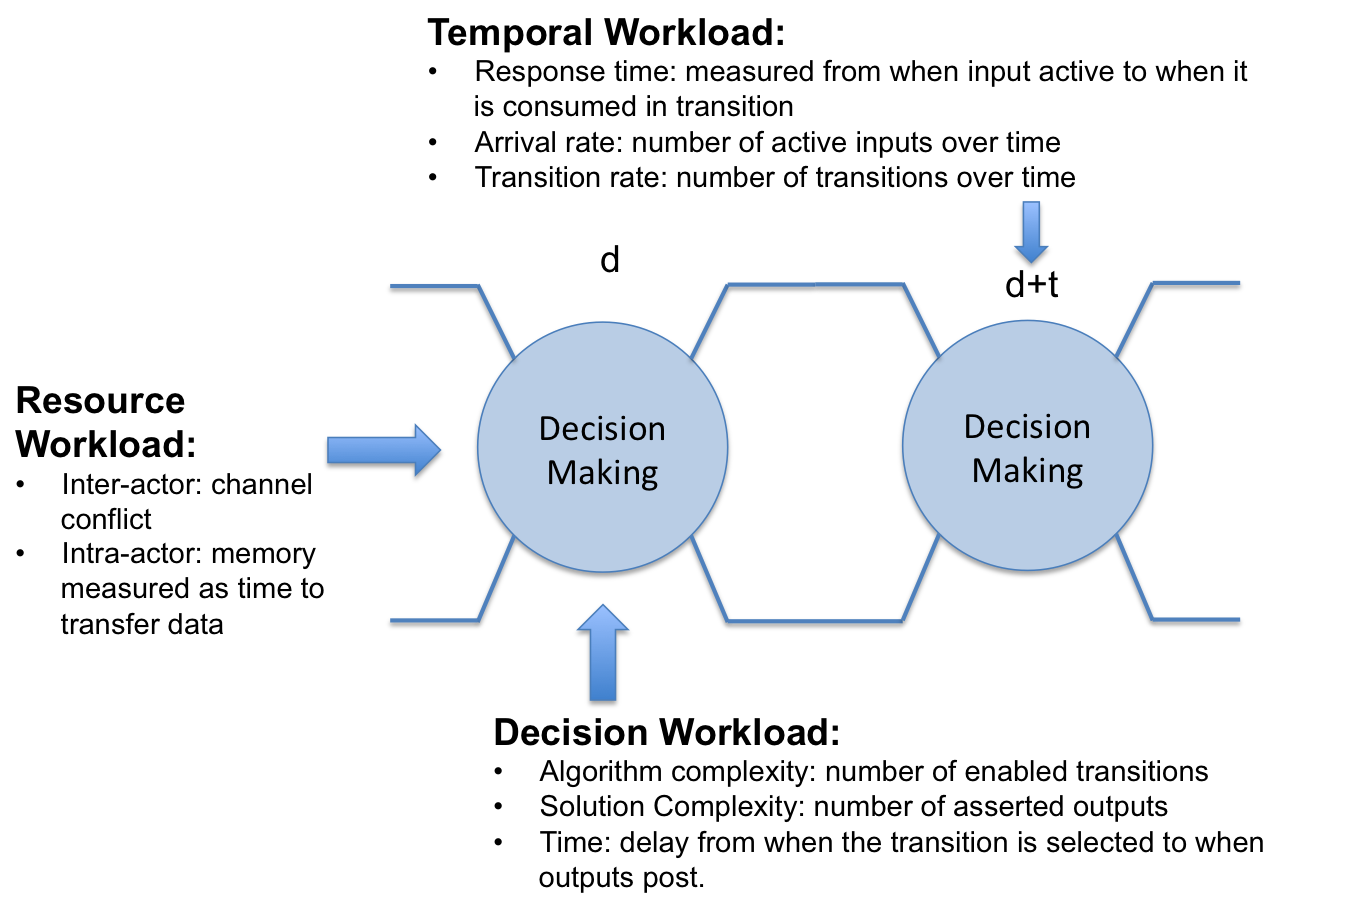
\includegraphics[height=2.5in]{WorkloadMetrics.png}
\caption{Workload in the model.}
\label{fig:WorkloadMetrics}
\end{figure}

\subsection{Resource Metrics}
Cognitive workload is separated into both inter-actor communication and actor memory load. JPF listens to the output of the state transitions and records outputs to $\Omega_{\rm men}$.  JPF also listens to all channel reads, noting how many communications are on the visual and auditory input channel, identified by the labeled edges of the DiTG, of each actor. 


\subsection{Decision Metrics}
Algorithmic workload can be broken down into the timing, the complexity of the algorithm, and the complexity of the solution. JPF is instrumented to measure timing as the time between a transition becomes active and when it fires.  JPF is also instrumented to count the number of enabled transitions in each state as it is visited, giving us an $O(n)$ estimate of how the number of choices affects workload.   Finally, JPF is instrumented to count the number of output signals generated ($\Sigma_{\rm team}$), yielding an $O(n)$ estimate for the complexity of computing the required outputs of a state given its inputs.

\subsection{Temporal Metrics}
Temporal workload includes three metrics: operations tempo, arrival rate, and response time.  JPF measures the average op-tempo counting how many transitions occur over a course of the simulation. JPF measures arrival rate by tracking the rate at which inputs become active. Finally, JPF measures response time by measuring the time from when an input goes active to the point when it is read by the actor.
